\section{Durchführung}
\label{sec:Durchführung}

\begin{figure}
    \centering
    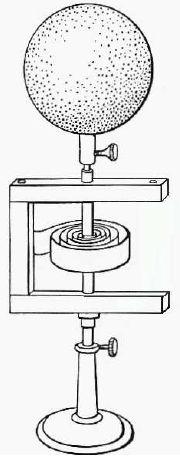
\includegraphics[height=6cm]{data/Bild_1.png}
    \caption{Aufbau}
    \label{fig:aufbau}
\end{figure}

Der grundlegende Aufbau ist in der kompletten Versuchsreihe gleichbleibend. Auf die Halterung, auf die im Bild\ref{fig:aufbau} die Kugel
montiert ist, werden im Folgenden alle zu untersuchenden Körper befestigt. 

\subsection{Bestimmung der Winkelrichtgröße $D$}

Um die Winkelrichtgröße $D$ zu bestimmen, wird unter die Halterung für den Körper eine Scheibe gelegt, auf der der Auslenkungswinkel 
abgelesen werden kann. In die Halterung wird anstelle der Kugel eine Stange waagerecht befestigt, die in deren Mitte verschraubt wird.
Die Stange hat einen Durchmesser von 0,5$\si{\centi\meter}$ und ist 60$\si{\centi\meter}$ lang. An dieser wird 10$\si{\centi\meter}$
von der Drehachse entfernt ein Newtonmeter angebracht, welches immer senkrecht zur Stange ausgerichtet ist. An dem Newtonmeter 
angreifend wird die Stange ausgelenkt. Dies wird in 10$\si{\degree}$-Schritten von 20$\si{\degree}$ bis 90$\si{\degree}$ gemacht.
Dabei wird jeweils die wirkende Kraft notiert, die bei der bestimmten Auslenkung wirkt. 

\subsection{Bestimmung des Eigenträgheitsmoments}

Hierbei wird die selbe Stange verwendet. Auf beiden Seiten wird jeweils eine Masse $m=223,3\si{\gram}$ in gleichem Abstand zur 
Drehachse montiert. Die Stange wird dann um einen kleinen Winkel ausgelenkt und losgelassen. Es wird die Periodendauer der Schwingung
mit einer Stoppuhr gemessen und notiert. Der Versuch wird mit zehn unterschiedlichen Abständen der Gewichte zur Drehachse durchgeführt.

\subsection{Bestimmung unterschiedlicher Trägheitsmomente}
\begin{figure}
    \centering
    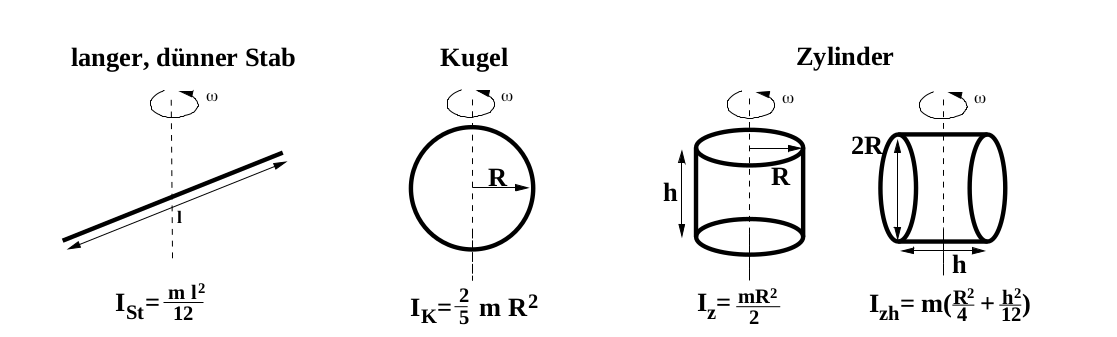
\includegraphics[height=6cm]{data/Probekoerper}
    \caption{Verschiedene Zylinder}
    \label{fig:Probekoerper}
\end{figure}


\begin{figure}
    \centering
    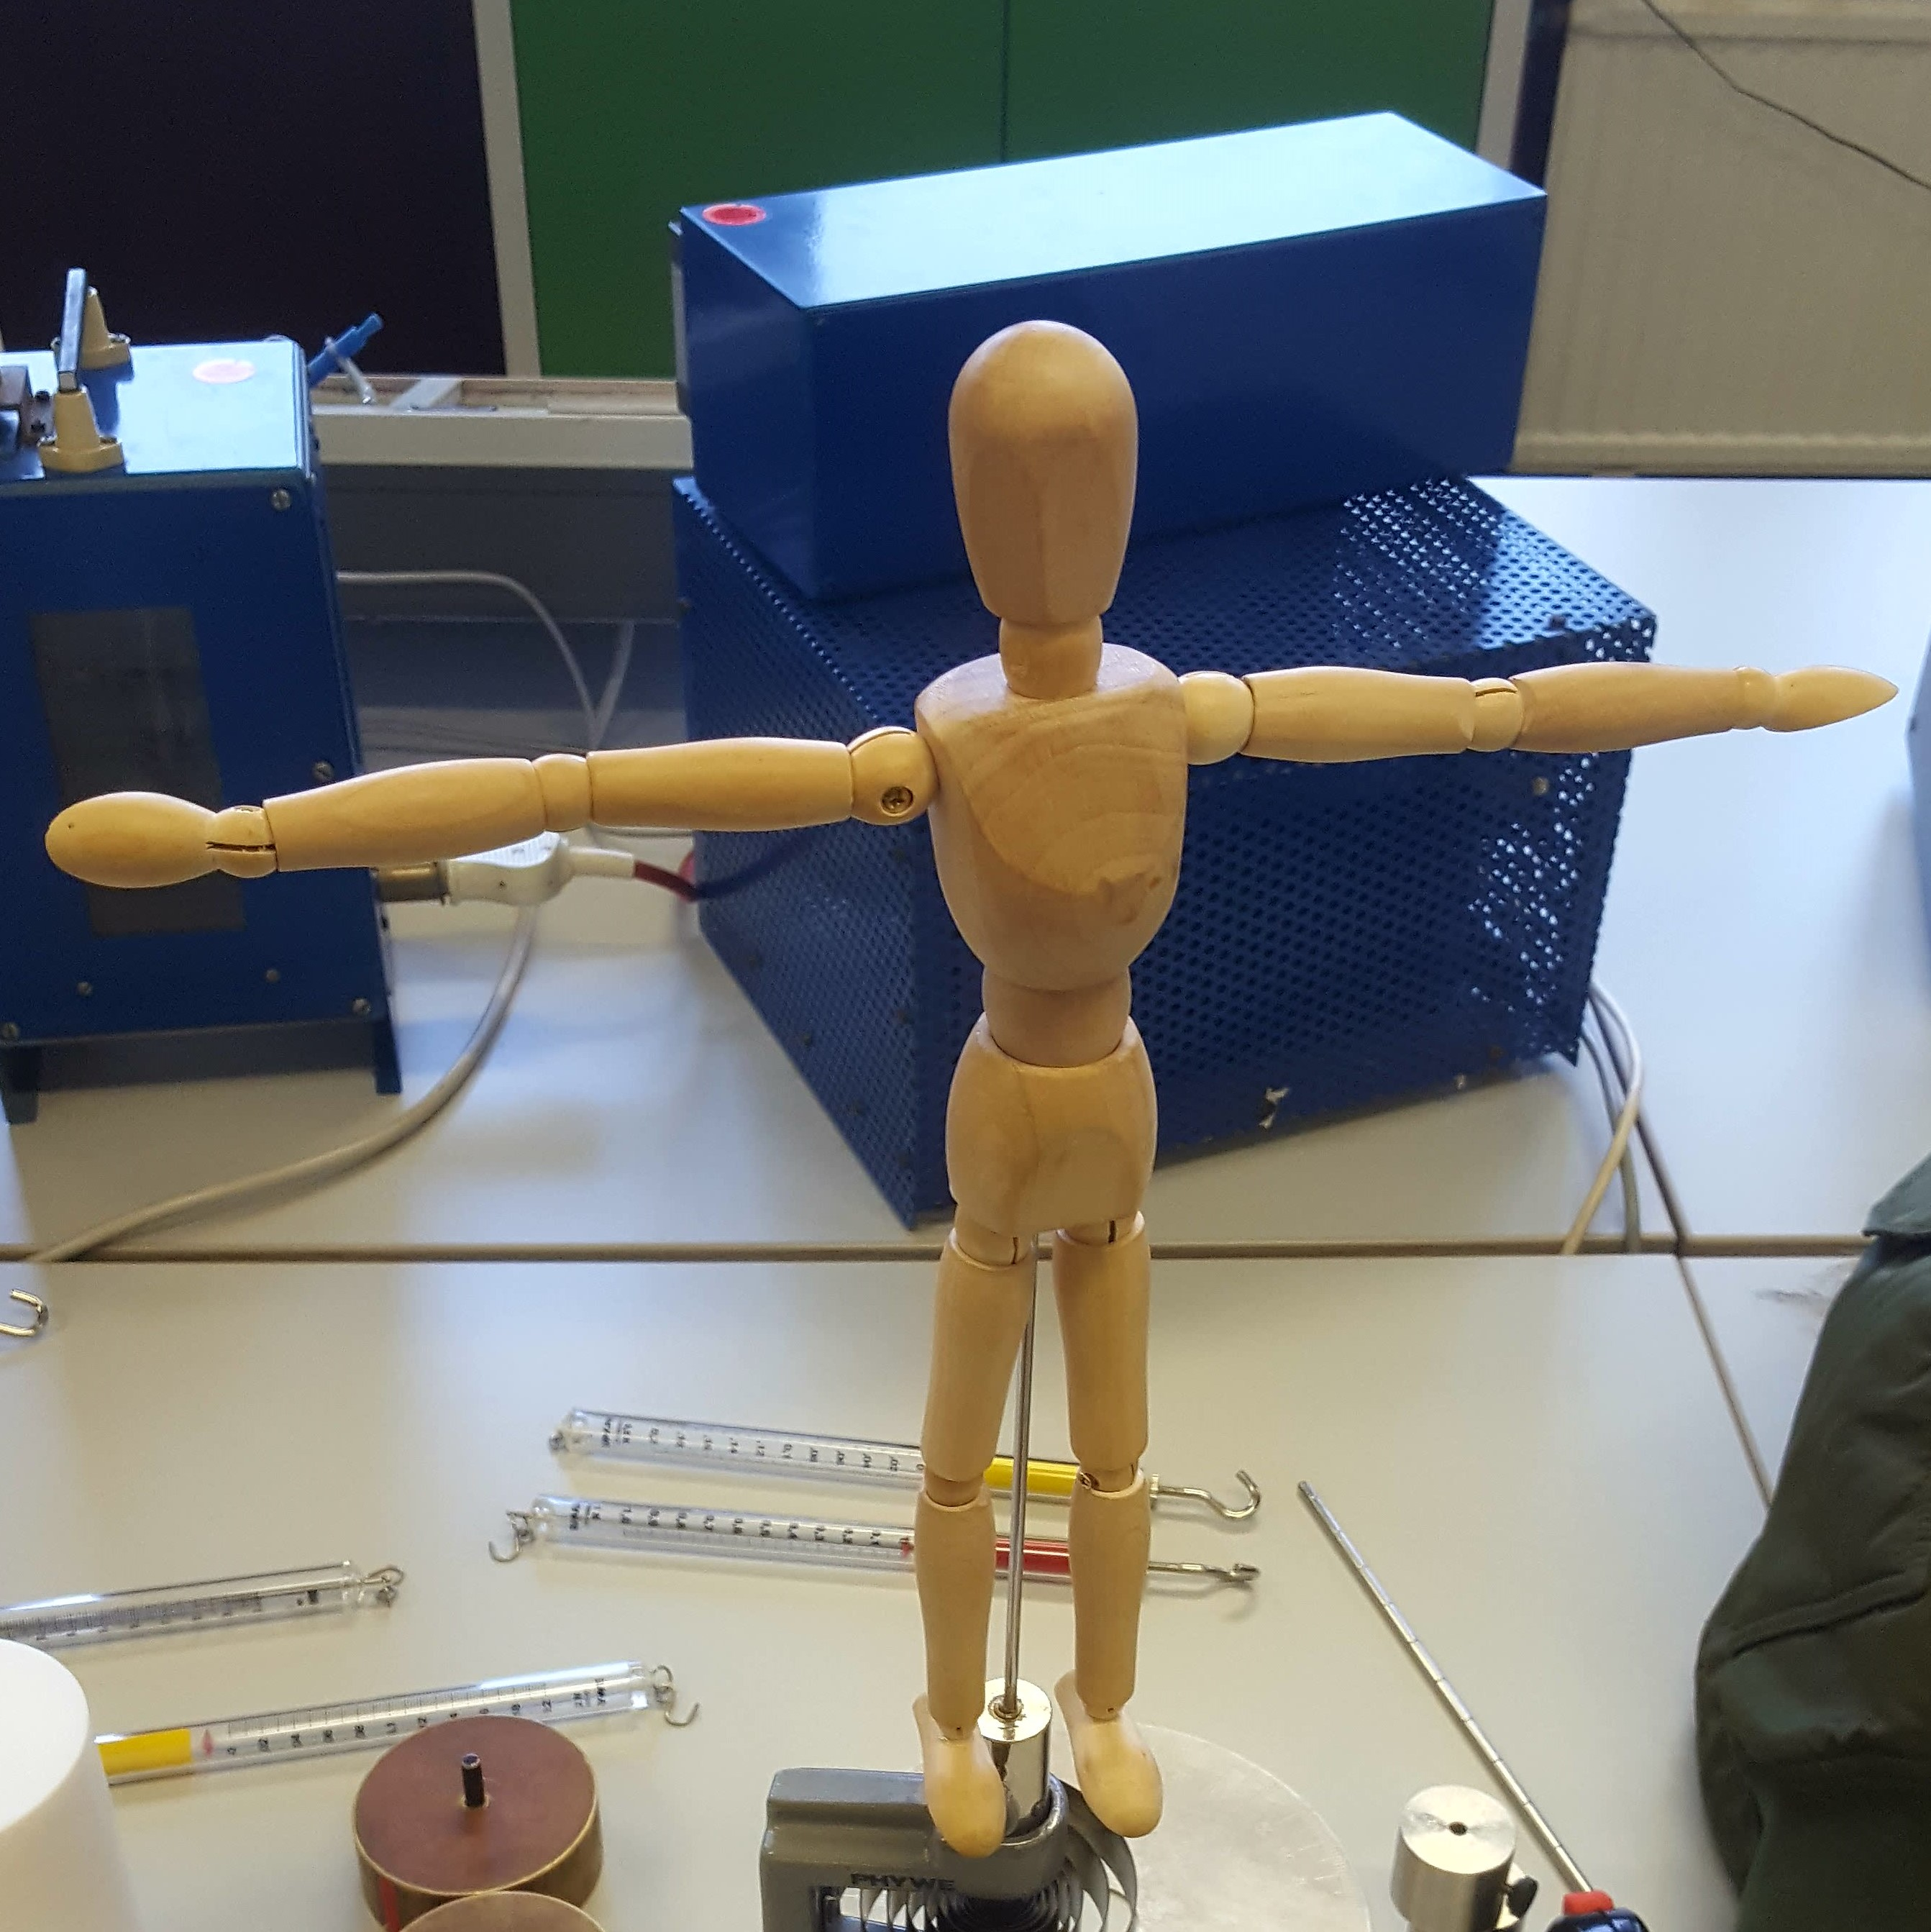
\includegraphics[height=6cm]{data/puppe_2}
    \caption{Puppe in Pos. 1}
    \label{fig:puppe_2}
\end{figure}

\begin{figure}
    \centering
    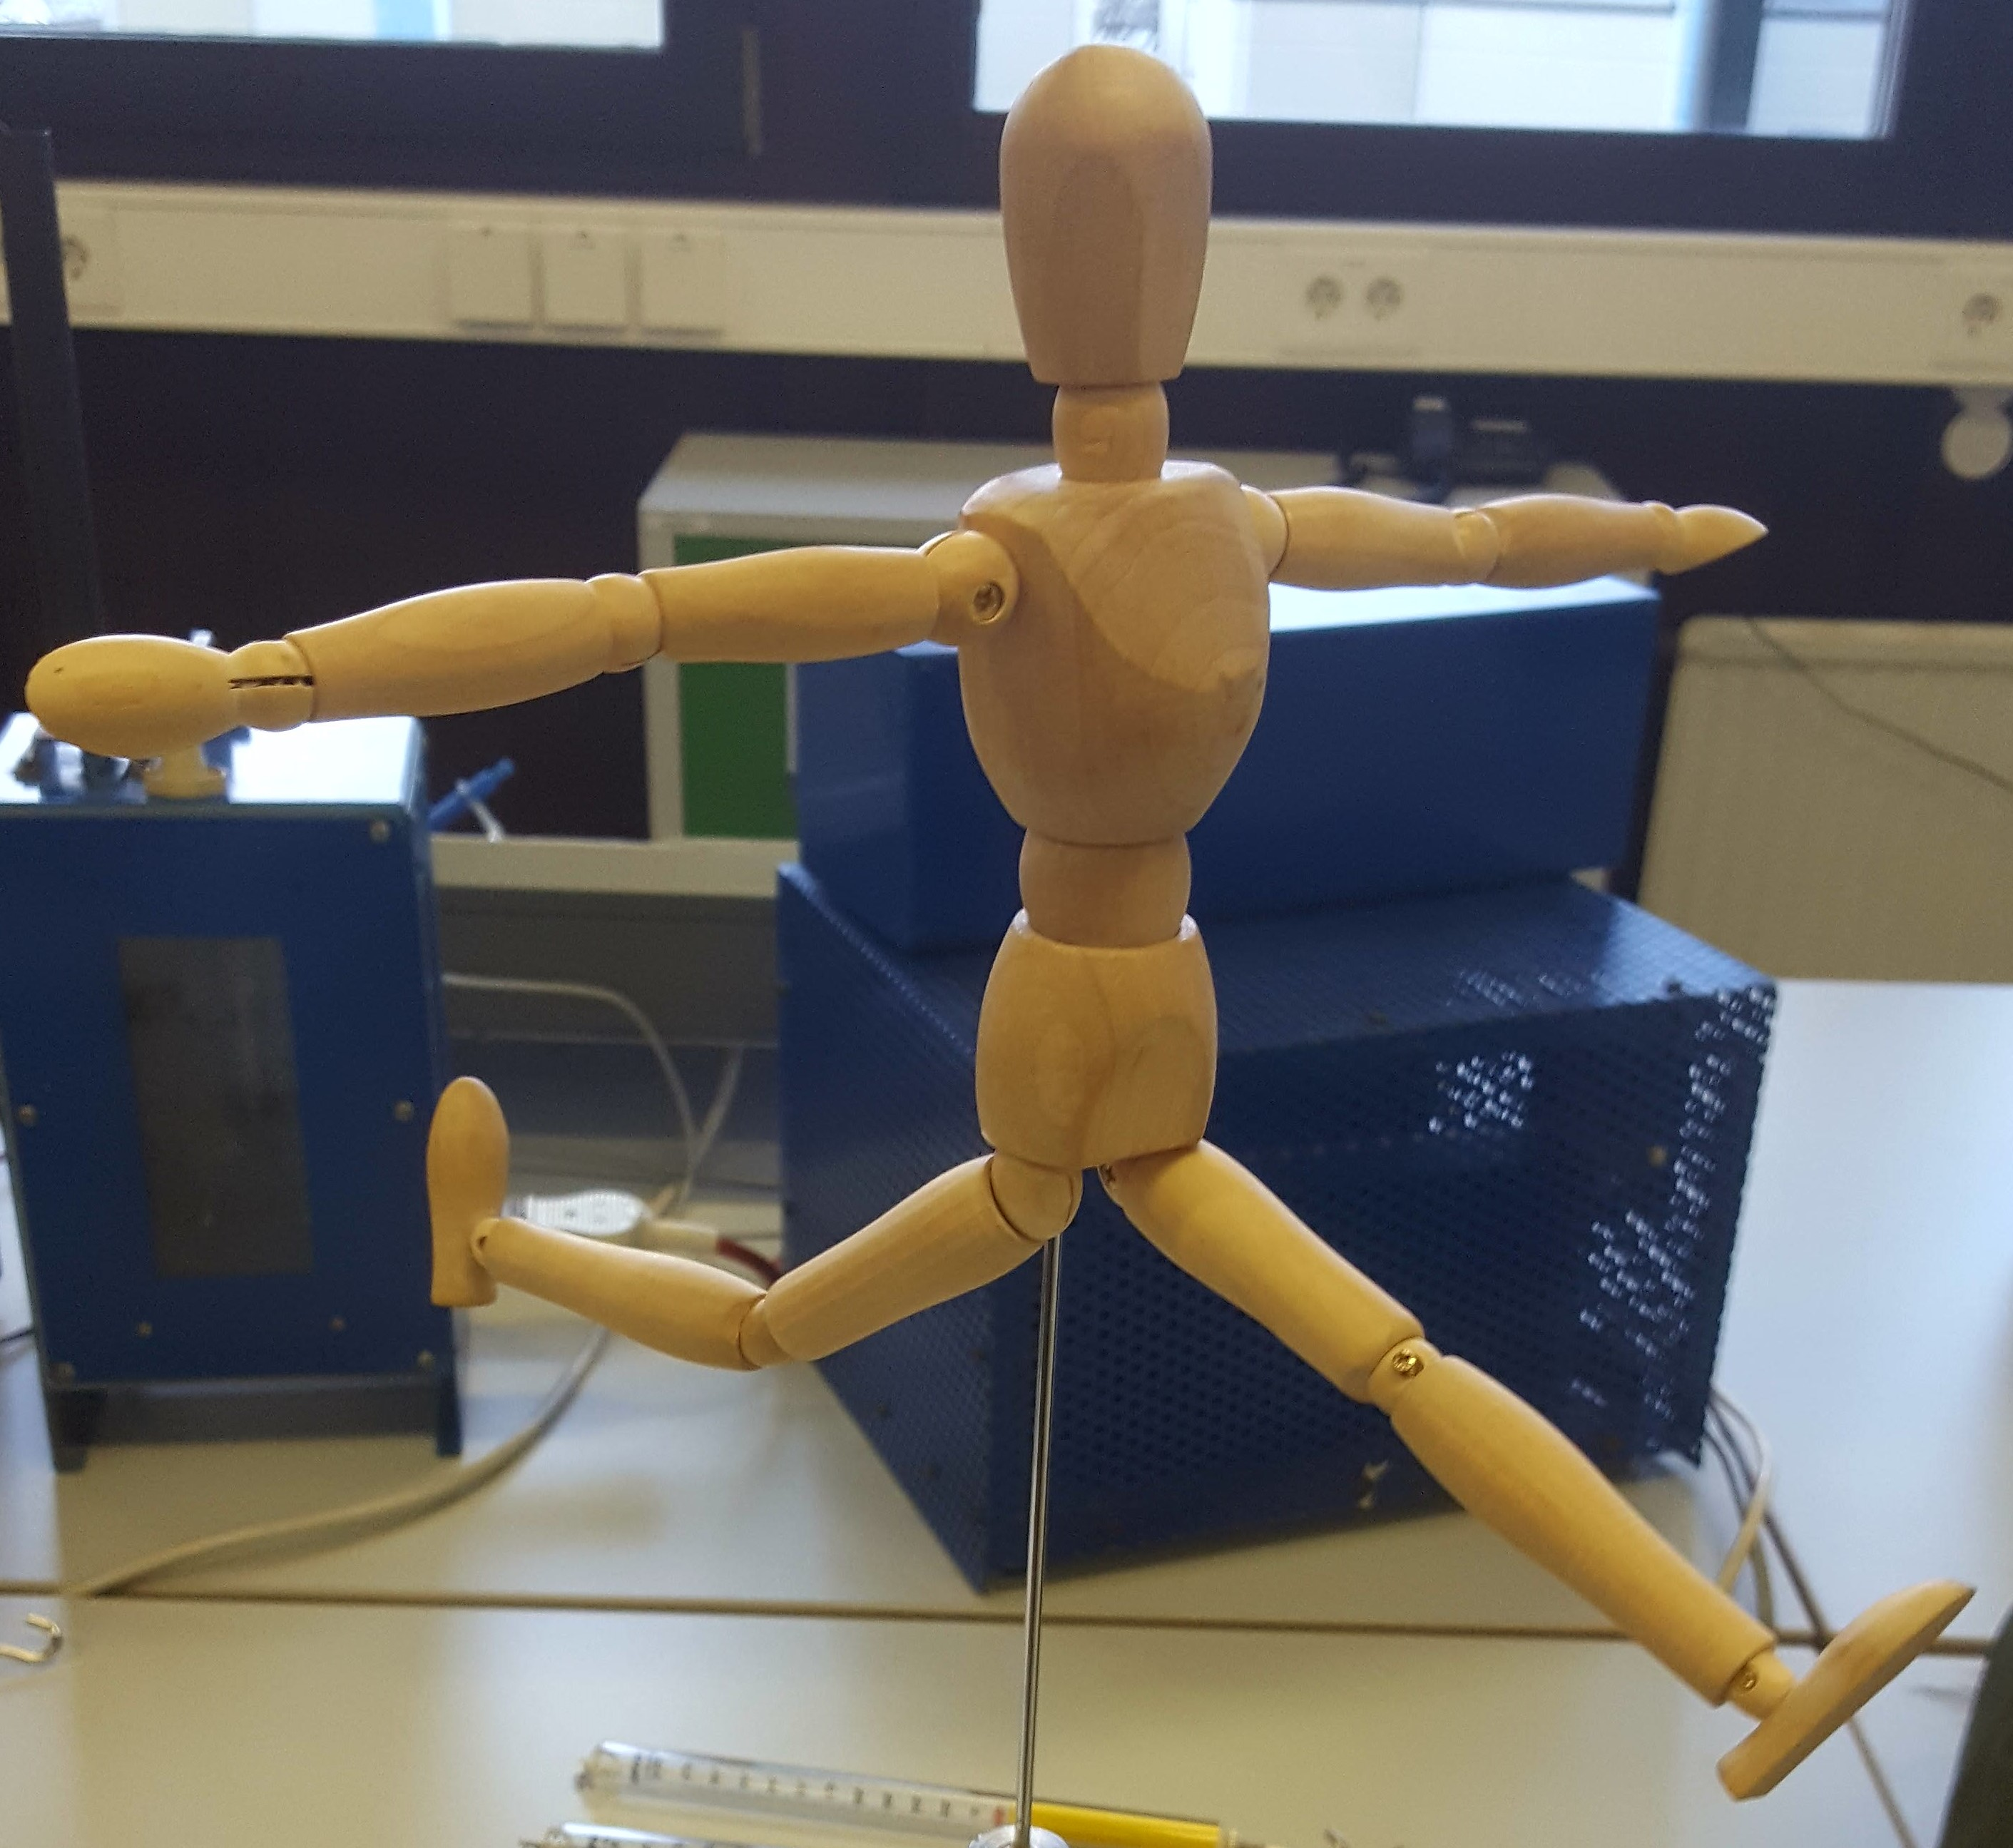
\includegraphics[height=6cm]{data/puppe_1}
    \caption{Puppe in Pos. 2}
    \label{fig:puppe_1}
\end{figure}



Die drei zu untersuchenden Körper werden jeweils anstelle der Kugel, wie sie in abb\ref{fig:aufbau} zu sehen ist, montiert.
Bei den Körpern handelt es sich um zwei identische Zylinder mit unterschiedlichen Drehachsen und einer Holzpuppe, die in 
Abb\ref{fig:puppe_2} und Abb\ref{fig:puppe_1} zu sehen ist. 

Einer der beiden Zylinder wird so verschraubt, dass er sich um seine Symmetrieachse dreht, der andere so, dass die Drehachse senkrecht
zur Symmetrieachse durch den Schwerpunkt verläuft, siehe Bild\ref{fig:Probekoerper}. Der Versuch wird für die Puppe in zwei 
verschiedenen Positionen durchgeführt. In Bild\ref{fig:puppe_2} und Bild\ref{fig:puppe_1} sind deren genaue Ausrichtungen gezeigt. 

Die Durchführung selbst ist für alle Körper gleich. Der jeweilige Körper wird am Aufbau fest montiert, so dass nur eine Drehung des 
Körpers über die Torsionsfeder möglich ist. Der Körper wird dann um einen kleinen Winkel ausgelenkt und losgelassen. Wie beim berechnen
des Eigenträgheitsmoments wird hierbei die Periodendauer der Schwingung mit einer Stoppuhr gemessen. Dabei werden für jeden Körper 
fünf Messungen der Periodendauer vorgenommen. 


